% NeST Policy 1: dormant connection activation (single-card figure).
\documentclass[tikz,border=8pt]{standalone}
\usepackage{amsmath,amssymb,bm}
\usetikzlibrary{positioning,calc}
\begin{document}
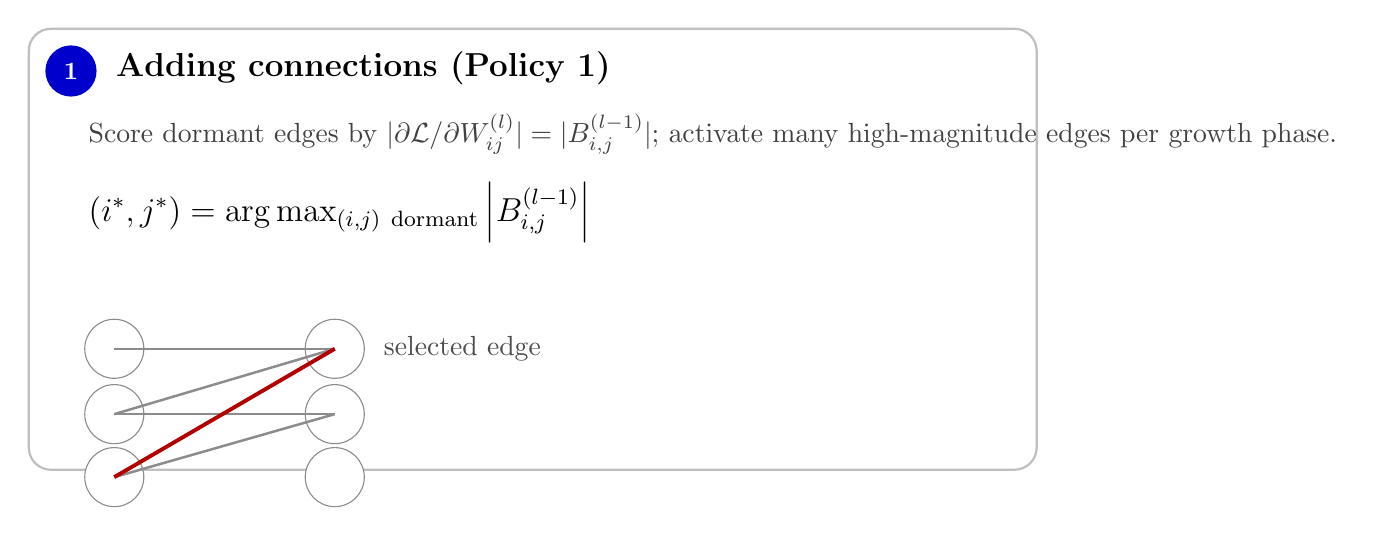
\begin{tikzpicture}[font=\sffamily]
\tikzset{
  card/.style={draw=black!25, rounded corners=8pt, fill=white, line width=0.8pt},
  nodec/.style={circle, draw=black!45, fill=white, minimum size=7.5mm, inner sep=0pt},
  edge/.style={draw=black!45, line width=0.9pt},
  sel/.style={draw=red!70!black, line width=1.4pt},
  stepnode/.style={circle, fill=blue!80!black, text=white, minimum size=6.5mm, inner sep=0pt, font=\bfseries\small}
}
\node[card, minimum width=12.8cm, minimum height=5.6cm, anchor=north west] (c) at (0,0) {};
\node[stepnode] at ($(c.north west)+(0.55,-0.55)$) {1};
\node[anchor=west, font=\bfseries\large] at ($(c.north west)+(1.0,-0.52)$) {Adding connections (Policy~1)};
\node[anchor=west, font=\normalsize, text=black!75] at ($(c.north west)+(0.65,-1.35)$)
  {Score dormant edges by $\lvert\partial\mathcal{L}/\partial W^{(l)}_{ij}\rvert=\lvert B^{(l-1)}_{i,j}\rvert$; activate many high-magnitude edges per growth phase.};
\node[anchor=west, font=\large] at ($(c.north west)+(0.65,-2.35)$)
  {$(i^\ast,j^\ast)=\arg\max_{(i,j)\ \mathrm{dormant}}\left\lvert B^{(l-1)}_{i,j}\right\rvert$};
\coordinate (a1) at ($(c.south west)+(1.1,1.55)$);
\coordinate (a2) at ($(c.south west)+(1.1,0.72)$);
\coordinate (a3) at ($(c.south west)+(1.1,-0.08)$);
\coordinate (b1) at ($(c.south west)+(3.9,1.55)$);
\coordinate (b2) at ($(c.south west)+(3.9,0.72)$);
\coordinate (b3) at ($(c.south west)+(3.9,-0.08)$);
\foreach \p in {a1,a2,a3,b1,b2,b3} \node[nodec] at (\p) {};
\draw[edge] (a1)--(b1);
\draw[edge] (a2)--(b1);
\draw[edge] (a2)--(b2);
\draw[edge] (a3)--(b2);
\draw[sel]  (a3)--(b1);
\node[anchor=west, font=\normalsize, text=black!70] at ($(b1)+(0.5,0)$) {selected edge};
\end{tikzpicture}
\end{document}
